\chapter{Graphical User Interfaces}
\label{chap:windows}

A \idx{command-line interface} (\idx{CLI}) is a method for communicating with the user through text. In contrast, a \idx{graphical user interface} (\idx{GUI}) extends the ways of communicating with the user to also include organising the screen space in windows, icons, and other visual elements, and a typical way to activate these elements are through a pointing device such as the mouse or by touch. Some of these elements may themselves be textual, and thus most operating systems offers access to a command-line interface in a window alongside other interface types.

Fsharp includes a number of implementations of graphical user interfaces, but at time of writing only \idx{WinForms} is supported on both the Microsoft .Net and the Mono platform, and hence, WinForms will be the subject of the following chapter.

WinForms is designed for \idx{event driven programs}, which spends most time waiting for the user to perform an action, called and event, and for each event has a set of predefined responses to be performed by the program. For example, Figure~\ref{fig:safariGui} shows the program Safari, which is a graphical user interface for accessing web-servers.
\begin{figure}
  \centering
  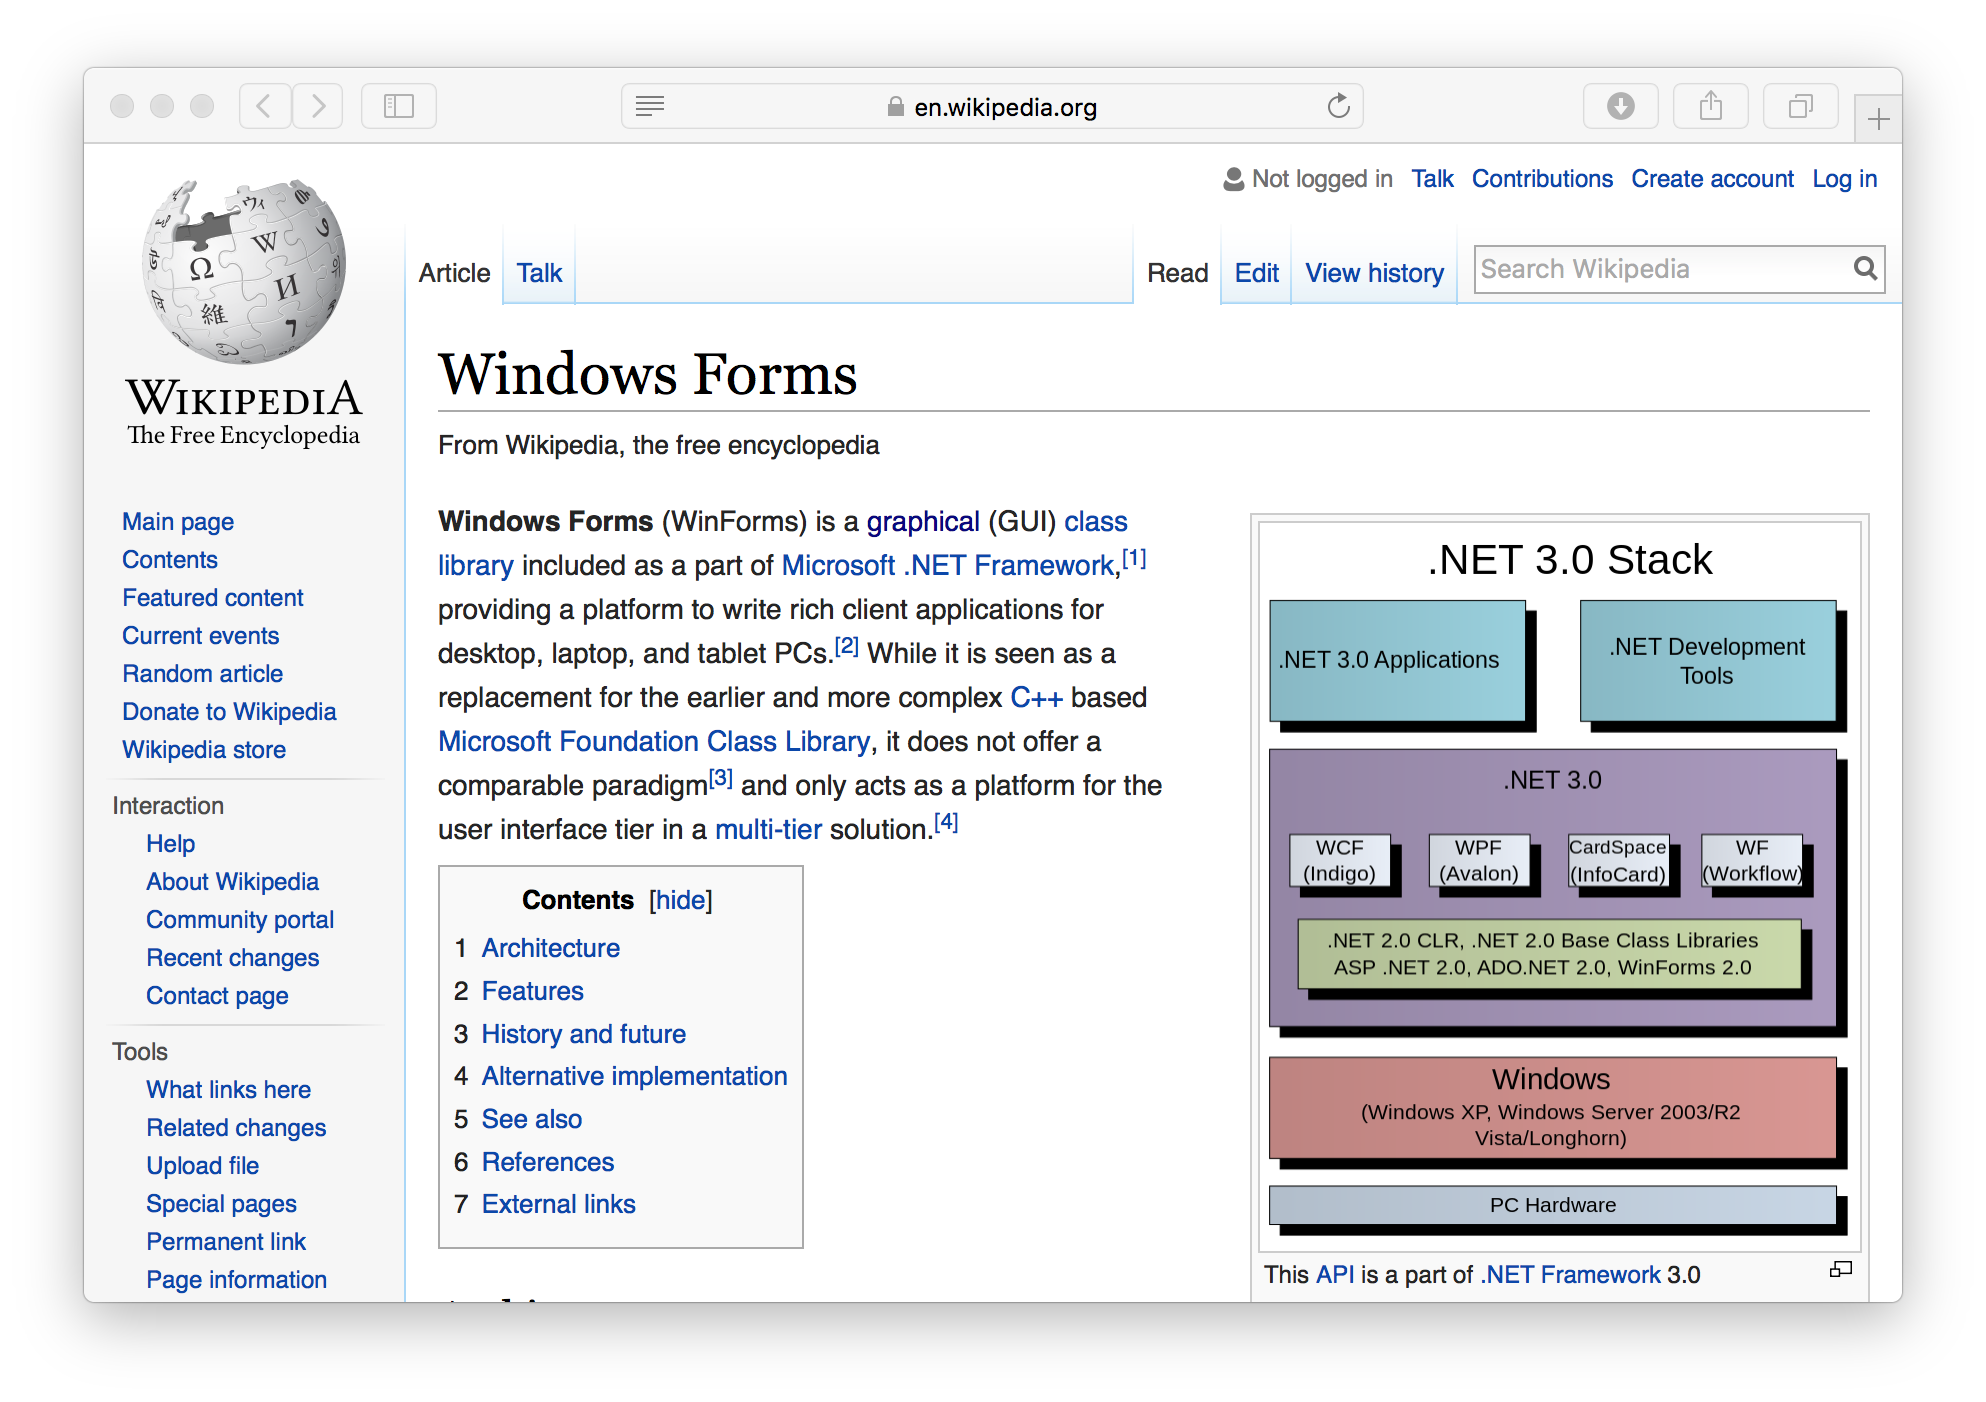
\includegraphics[width=0.6\textwidth]{safariWinForms}
  \caption{A web-browser is a graphical user interface for accessing a web-server and interacting with its services. Here the browser is showing the page \url{https://en.wikipedia.org/wiki/Windows_Forms} at time of writing.}
  \label{fig:safariGui}
\end{figure}
The program present information to the user in terms of text and images, and has areas that when activated by clicking with a mouse or similar allows the user to, e.g., go to other web-pages by type URL, to follow hyperlinks, and to generate new pages by entering search queries.

\section{Drawing primitives in Windows}
WinForms is based on two namespaces: \lstinline!System.Windows.Forms! and \lstinline!System.Drawing!. To start making a graphical display on the screen, the first thing to do is open a window, which acts as a reserved screen space for our output. With WinForms, this may be done as shown in Listing~\ref{winforms/openWindow}, and the result is shown in Figure~\ref{fig:openWindow}.
%
\fsCode{winforms/openWindow}{Create the window and turn over control to the operating system. Use \lstinline!win.Show()! on Microsoft Windows instead.}
%
\begin{figure}
  \centering
  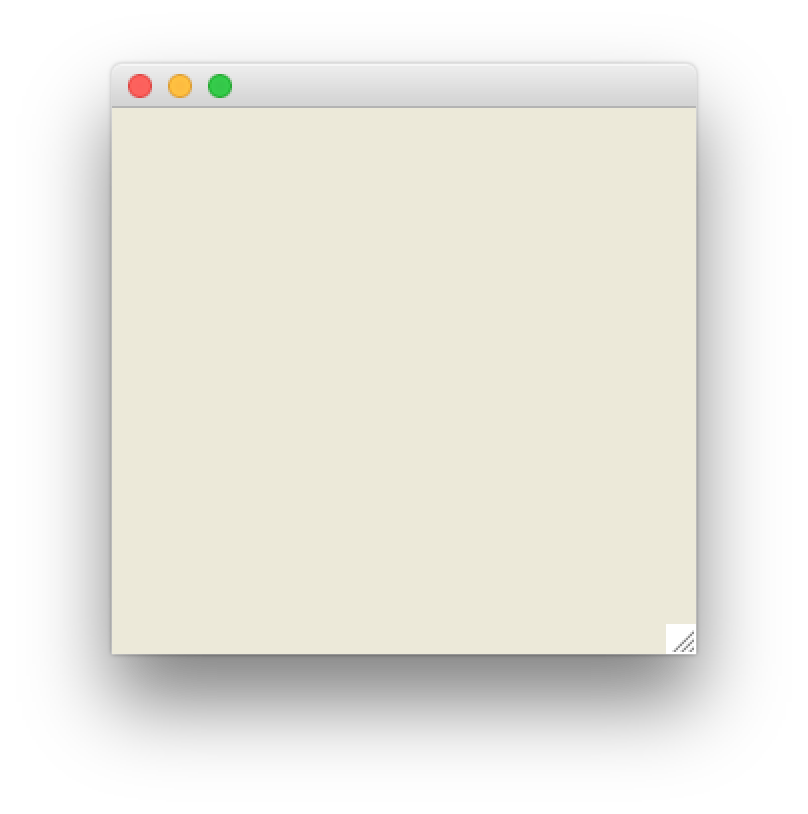
\includegraphics[width=0.6\textwidth]{openWindow}
  \caption{Result of running listing Listing~\ref{winforms/openWindow}.}
  \label{fig:openWindow}
\end{figure}
The \lstinline!new System.Windows.Forms.Form ()! creates an object (See Chapter~\ref{chap:oop}), but does not display the window on the screen. When the function \lstinline!System.Windows.Forms.Application.Run! is applied to the object, then the control is handed over to the WinForm's \idx{event-loop}, which continues until the window is closed by, e.g., pressing the icon designated by the operating system. On the mac OSX that is the red button in the top left corner of the window frame, and on Window it is the cross on the top right corner of the window frame.

The window, which WinForms calls a form, has a long list of \idx{methods} and \idx{properties}. E.g., the background color may be set by \lstinline!BackColor!, the title of the window may be set by \lstinline!Text!, and you may get and set the size of the window with the \lstinline!Size!. This is demonstrated in Listing
%
\fsCode{winforms/windowAttributes}{Create the window and changing its properties.}
%
\begin{figure}
  \centering
  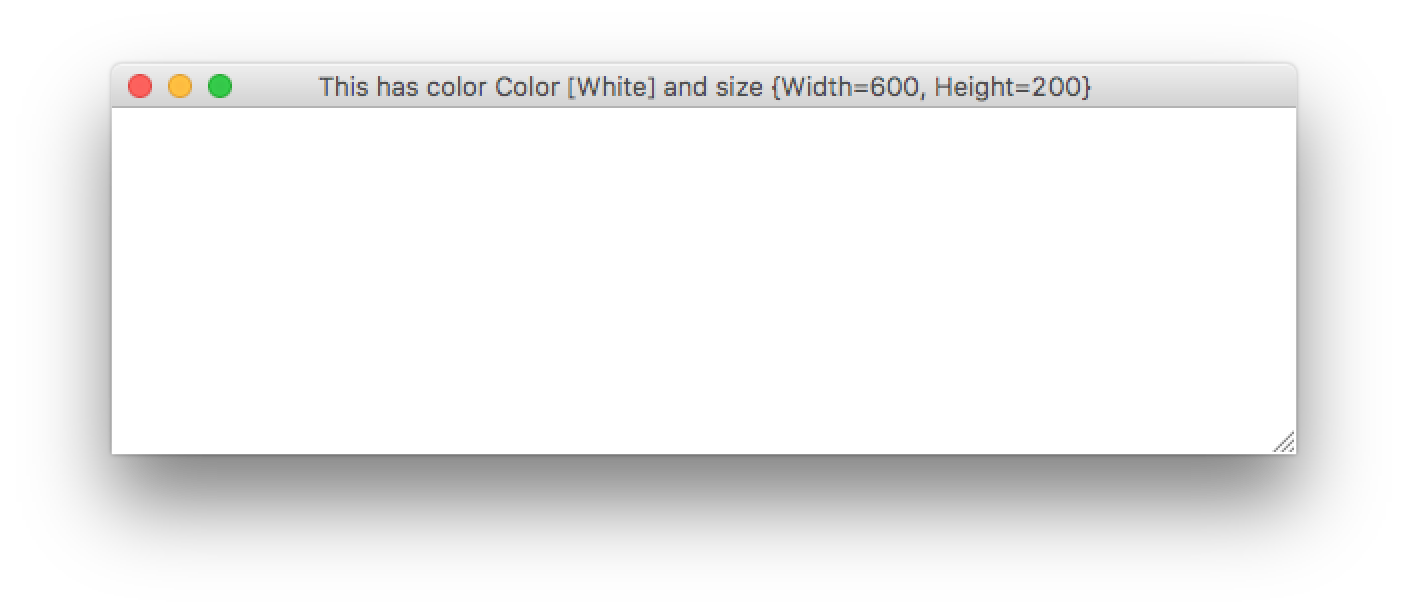
\includegraphics[width=0.6\textwidth]{windowAttributes}
  \caption{Result of running listing Listing~\ref{winforms/windowAttributes}.}
  \label{fig:openWindow}
\end{figure}
These properties have been programmed as \idx{accessors} implying that they may used as mutable variables. The \idx{\lstinline{System.Drawing.Color}} is a general structure for specifying colors as 4 channels: alpha, red, green, blue, where each channel is an 8 bit unsigned integer, where the alpha channel specifies the transparency of a color, where values 0--255 denotes the range of fully transparent to fully opaque, and the remaining channels denote the amount of red, green, and blue where 0 is none and 255 is full intensity. Any color may be created using the \lstinline!FromArgb! method, e.g., an opaque red is given by \lstinline!System.Drawing.Color.FromArgb (255, 255, 0, 0)!. There are also many build-in colors, e.g., the same red color is also a known color and may be obtained as \lstinline!System.Drawing.Color.Red!. For a given color, then the 4 alpha, red, green, and blue channel's values may be obtained as the \lstinline!A!, \lstinline!R!, \lstinline!G!, \lstinline!B!, see Listing~\ref{drawingColors}
%
\fs{drawingColors}{Defining colors and accessing their values.}
%
The \lstinline!System.Drawing.Size! is a general structure for specifying sizes as height and width pair of integers.

WinForms supports drawing of simple graphics primitives. Simple examples are \lstinline!System.Drawing.Pen! to specify the color to be drawn, \lstinline!System.Drawing.Point! to specify a pair of coordinates, and \lstinline!System.Drawing.Graphics.DrawLine!. \lstinline!DrawLine! is different than the previous examples since it must be related to a specific device, and it is typically accessed as an event. Displaying graphics in WinForms is performed as the reaction to an event. E.g., windows are created by the program, moved, minimized, occluded by other windows, resized, etc., by the user or the program, and each action may require that the content of the window is refreshed. Thus, we must create a function that WinForms can call, when it determines that the content needs to be redrawn. This is known as a \idx{call-back function}, and it is added to an existing form using the \lstinline!Paint.Add! function. As an example, consider the problem of draw a triangle in a window. For this we need to make a function that can draw a triangle not once, but any time WinForms determines it necessary to draw and redraw the triangle. This is done in Listing~\ref{winforms/triangle}.
%
\fsCode{winforms/triangle}{Create the window and changing its properties.}
%
\begin{figure}
  \centering
  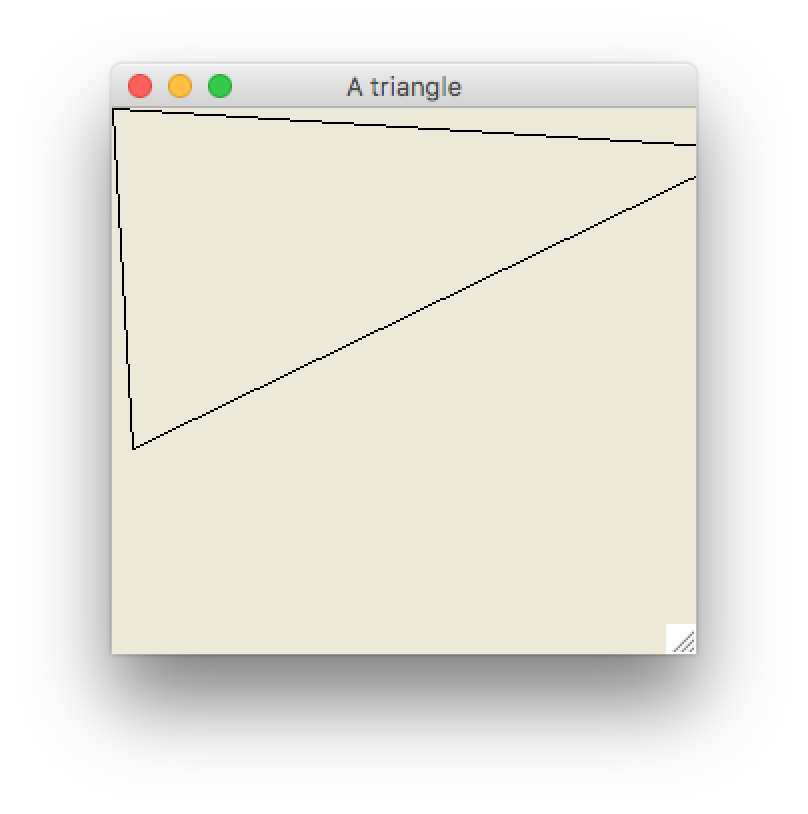
\includegraphics[width=0.6\textwidth]{triangle}
  \caption{Result of running listing Listing~\ref{winforms/triangle}.}
  \label{fig:triangle}
\end{figure}
A walk-through of the code is as follows: First we create an array of points and a pen color, then we create a pen and a window. The method for drawing the triangle is added as an anonymous function using the created window's \lstinline!Paint.Add! method. This function is to be called as a response to a paint event, and takes a \lstinline!PaintEventArgs! object, which includes the System.Drawing.Graphics object. Since this object will be related to a specific device, when \lstinline!Paint! is called then we may call the \lstinline!DrawLine! function to sequentially draw lines between our array of points. Finally, we hand the form to the event-loop, which as one of the earliest events will open the window and call the \lstinline!Paint! function we have associated with the form.

%
\fsCode{winforms/triangleOrganized}{Create the window and changing its properties.}
%
\begin{figure}
  \centering
  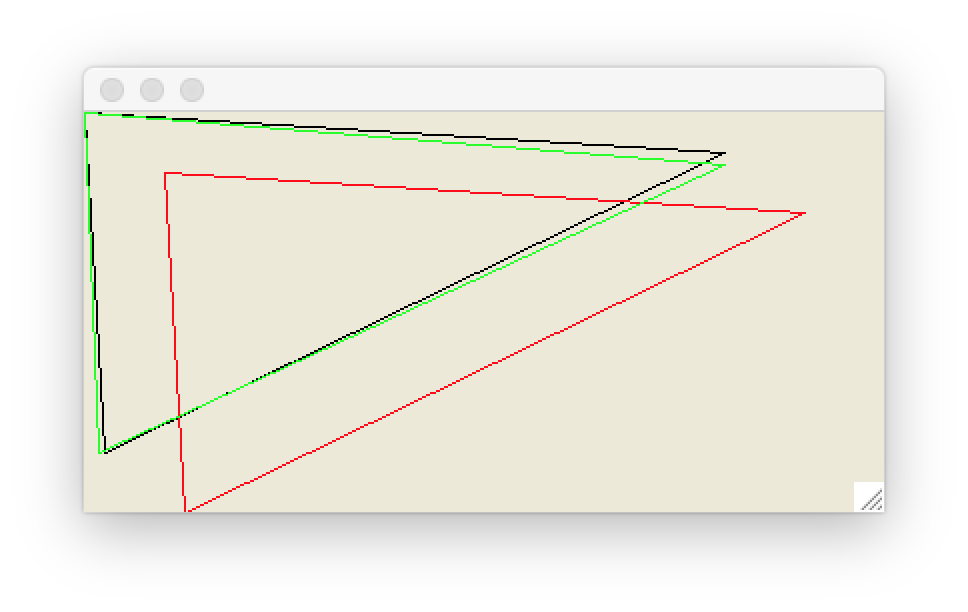
\includegraphics[width=0.6\textwidth]{triangleOrganized}
  \caption{Result of running listing Listing~\ref{winforms/triangleOrganized}.}
  \label{fig:triangleOrganized}
\end{figure}
\jon{requires the introduction of type declarations.}\jon{Remember to talk about pen width.}

%
\fsCode[lastline=38]{winforms/transformWindows}{Create the window and changing its properties: top part.}
\fsCode[firstline=40]{winforms/transformWindows}{Create the window and changing its properties: bottom part.}
%
\begin{figure}
  \centering
  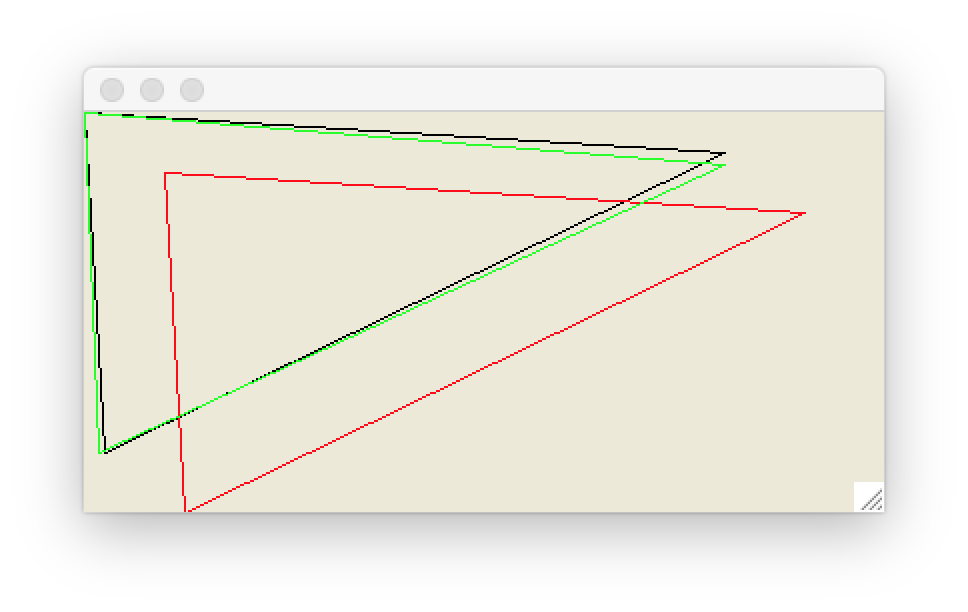
\includegraphics[width=0.6\textwidth]{transformWindows}
  \caption{Result of running listing Listing~\ref{winforms/transformWindows}.}
  \label{fig:transformWindow}
\end{figure}

\begin{problem}
  Given a triangle produce a Mandela drawing, where $n$ rotated versions of the triangle is drawn around its center of mass.
\end{problem}
%
\fsCode[firstline=40]{winforms/rotationalSymmetry}{Create the window and changing its properties.}
%
\begin{figure}
  \centering
  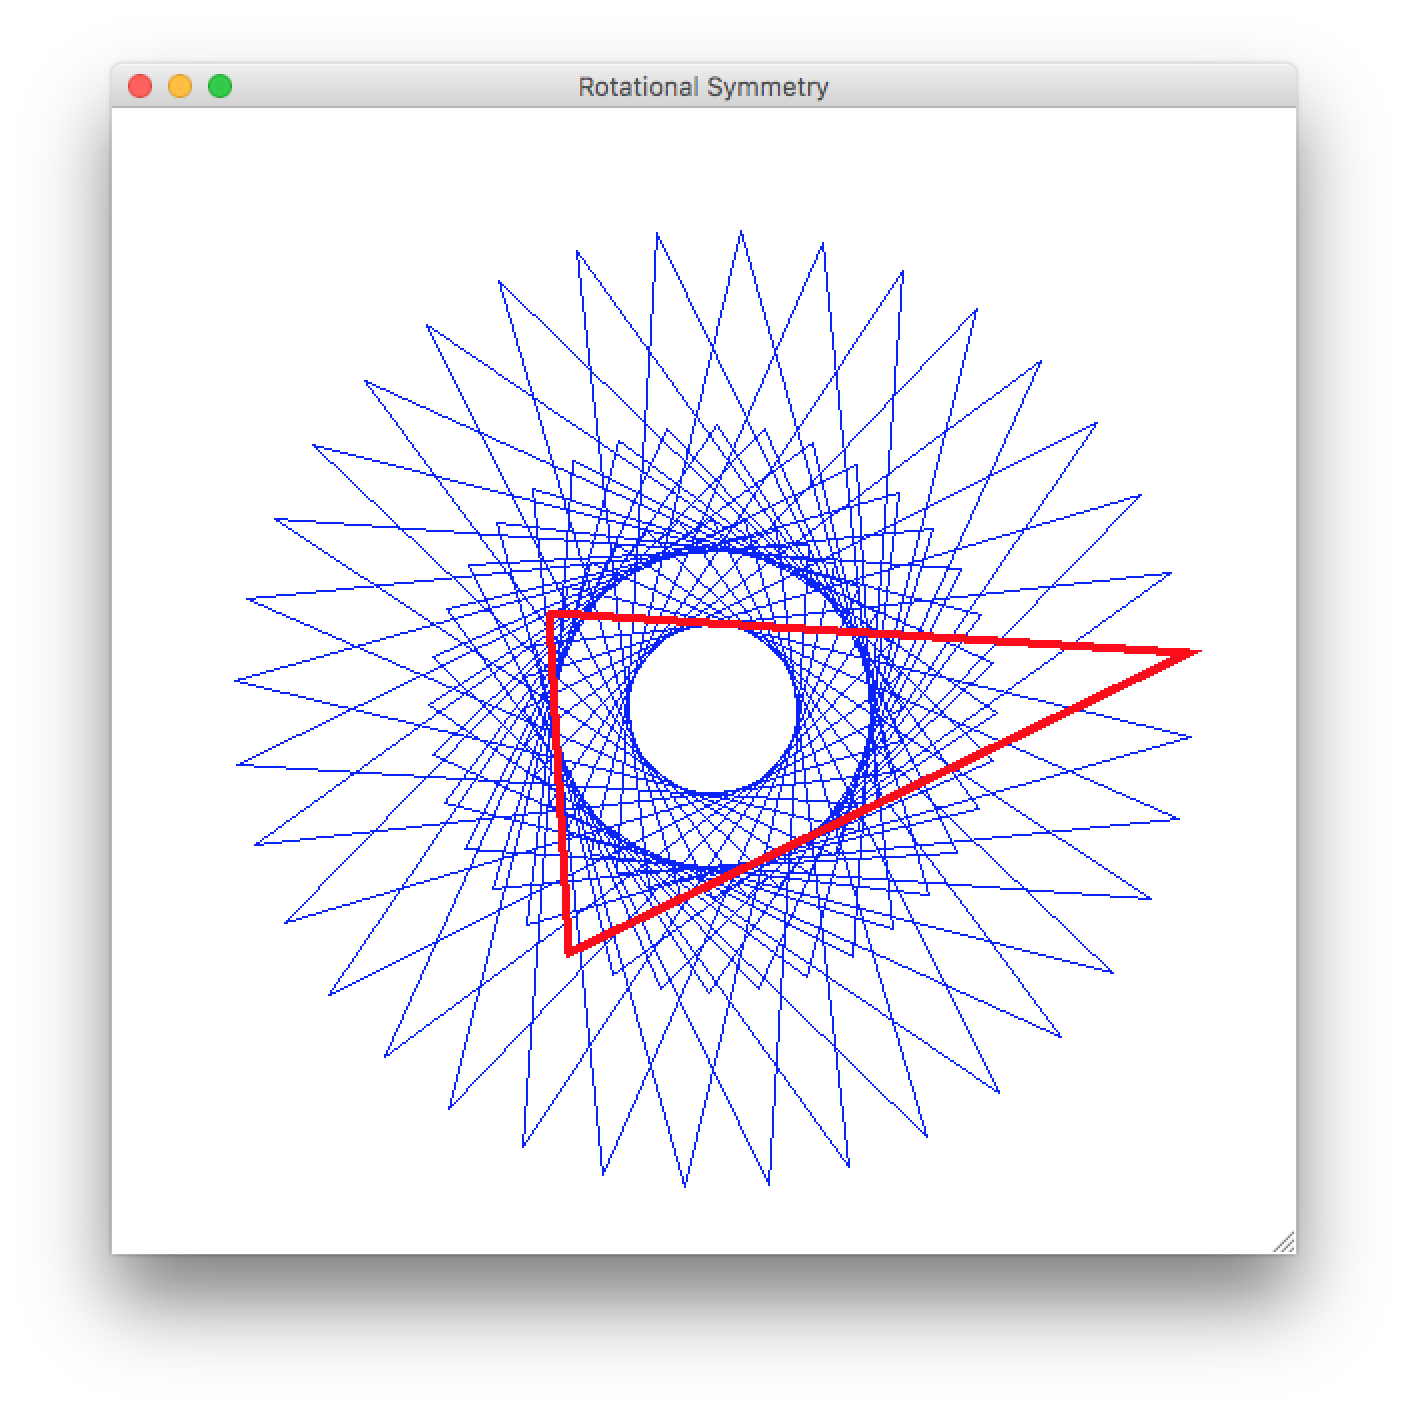
\includegraphics[width=0.8\textwidth]{rotationalSymmetry}
  \caption{Result of running listing Listing~\ref{winforms/rotationalSymmetry}.}
  \label{fig: rotationalSymmetry}
\end{figure}

\jon{Add other things to draw: filled stuff, clearing, circles, text}

\section{Buttons and stuff}

\dots

%%% Local Variables:
%%% TeX-master: "fsharpNotes"
%%% End:
